% =============================================================================
% AI Workflow Section — StatsClaw / OpenClaw Framework
% Requires: tikz, amsmath, amssymb, booktabs, xcolor, enumitem, hyperref
% TikZ libraries: positioning, arrows.meta, shapes.geometric, calc, fit,
%                  decorations.pathreplacing, backgrounds, shadows
% =============================================================================

\usepackage{tikz}
\usetikzlibrary{positioning, arrows.meta, shapes.geometric, calc, fit,
                 decorations.pathreplacing, backgrounds, shadows, chains}
\usepackage{amsmath,amssymb}
\usepackage{booktabs}
\usepackage{enumitem}

% ---------- color palette ----------
\definecolor{cPrimary}{HTML}{1565C0}      % deep blue
\definecolor{cSecondary}{HTML}{0D47A1}    % darker blue
\definecolor{cAccent}{HTML}{FF6F00}       % amber
\definecolor{cSuccess}{HTML}{2E7D32}      % green
\definecolor{cDanger}{HTML}{C62828}       % red
\definecolor{cLight}{HTML}{E3F2FD}        % light blue bg
\definecolor{cLightGreen}{HTML}{E8F5E9}   % light green bg
\definecolor{cLightRed}{HTML}{FFEBEE}     % light red bg
\definecolor{cLightAmber}{HTML}{FFF8E1}   % light amber bg
\definecolor{cGray}{HTML}{616161}         % mid gray
\definecolor{cLightGray}{HTML}{F5F5F5}    % very light gray
\definecolor{cCodePipe}{HTML}{1E88E5}     % code pipeline blue
\definecolor{cTestPipe}{HTML}{43A047}     % test pipeline green
\definecolor{cBridge}{HTML}{8E24AA}       % bridge purple
\definecolor{cConverge}{HTML}{E65100}     % convergence orange

% ---------- tikz styles ----------
\tikzset{
  agentbox/.style={
    draw=#1, fill=#1!8, rounded corners=3pt,
    minimum width=2.4cm, minimum height=0.85cm,
    font=\footnotesize\sffamily\bfseries, text=#1!90!black,
    drop shadow={shadow xshift=0.4pt, shadow yshift=-0.4pt, opacity=0.15}
  },
  artifact/.style={
    draw=cGray!60, fill=cLightGray, rounded corners=2pt,
    minimum width=1.8cm, minimum height=0.55cm,
    font=\scriptsize\ttfamily, text=cGray!90!black
  },
  signalbox/.style={
    draw=#1, fill=#1!10, rounded corners=2pt,
    minimum width=1.6cm, minimum height=0.5cm,
    font=\scriptsize\sffamily\bfseries, text=#1!85!black
  },
  pipelinelabel/.style={
    font=\scriptsize\sffamily\itshape, text=#1
  },
  arrowstyle/.style={
    -{Stealth[length=5pt, width=3.5pt]}, thick, color=#1
  },
  dashedarrow/.style={
    -{Stealth[length=5pt, width=3.5pt]}, thick, dashed, color=#1
  },
  gateline/.style={
    very thick, color=cDanger, dashed
  },
  statebox/.style={
    draw=cPrimary!60, fill=cLight, rounded corners=2pt,
    minimum width=1.4cm, minimum height=0.5cm,
    font=\scriptsize\sffamily, text=cPrimary!90!black
  },
  bigbox/.style={
    draw=#1!50, fill=#1!4, rounded corners=6pt, inner sep=8pt
  },
}


\section{AI Workflow}
\label{sec:ai-workflow}

We introduce \textbf{OpenClaw}, a multi-agent workflow framework that
orchestrates autonomous AI teammates to implement, validate, document,
and ship code changes across heterogeneous software projects. The
central architectural innovation is a \emph{dual-pipeline adversarial
verification} model: every non-trivial code change is simultaneously
processed through two informationally isolated pipelines---a
\textbf{code pipeline} and a \textbf{test pipeline}---whose outputs
are independently derived from a shared requirement but never
cross-contaminate. A dedicated convergence agent then cross-compares
the two pipelines' results; if both arrive at the same conclusion
independently, confidence in correctness is provably higher than in
any single-pipeline system.

This section formalizes the architecture, details each agent's role
and isolation constraints, specifies the state machine governing run
lifecycles, and describes the signal-based error recovery protocol.


% =====================================================================
\subsection{Architectural Overview}
\label{sec:arch-overview}
% =====================================================================

OpenClaw decomposes every code-change request into a directed acyclic
graph of agent tasks organized in four layers: \emph{analysis},
\emph{execution} (split into two isolated pipelines), \emph{recording},
and \emph{convergence}. A \emph{control} layer orchestrates the entire
process. Figure~\ref{fig:arch-overview} illustrates the full
architecture.

\begin{figure}[!t]
\centering
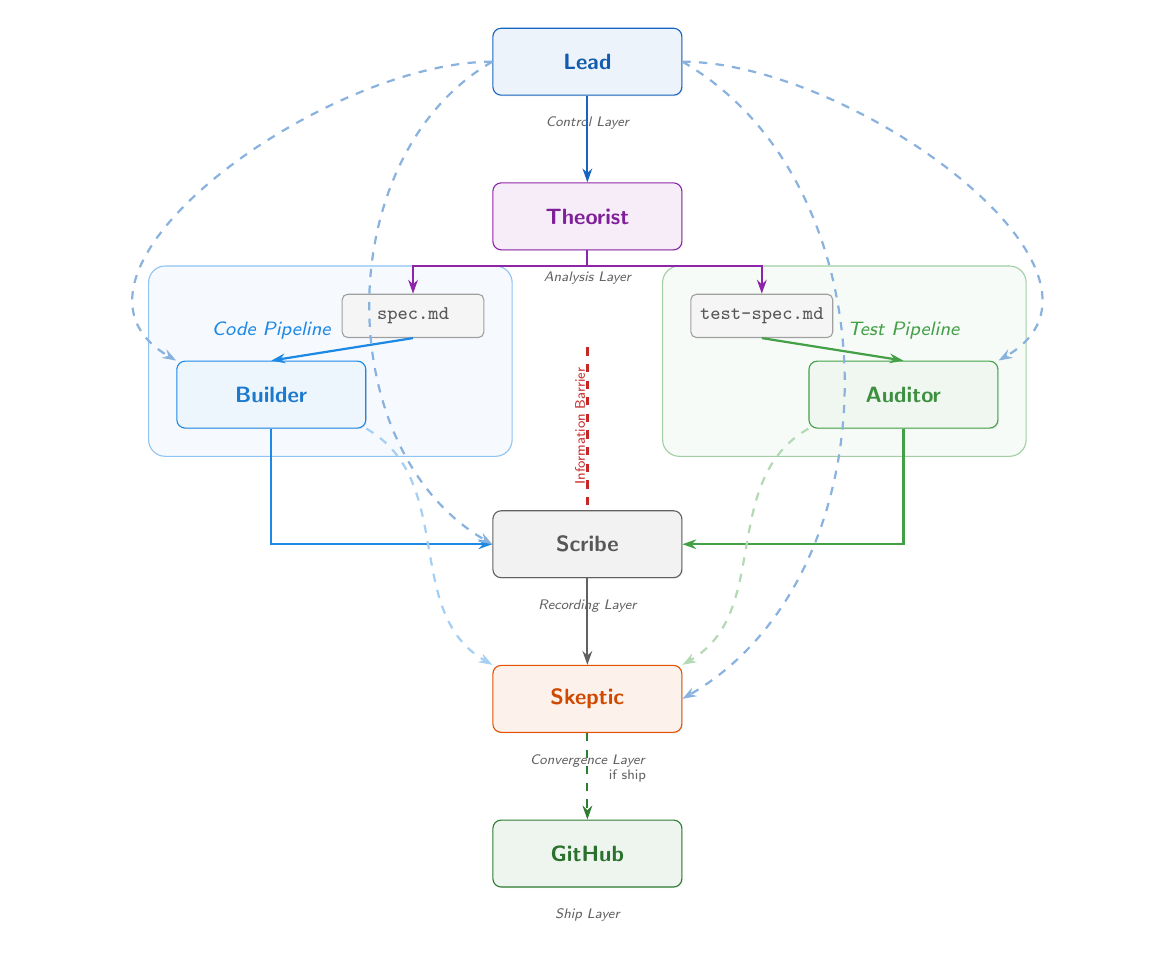
\begin{tikzpicture}[node distance=1.0cm and 1.5cm]

% ---- Control layer ----
\node[agentbox=cPrimary] (lead) {\textsf{Lead}};
\node[below=0.15cm of lead, font=\tiny\sffamily\itshape, text=cGray]
  (leadlabel) {Control Layer};

% ---- Analysis layer ----
\node[agentbox=cBridge, below=1.1cm of lead] (theorist) {\textsf{Theorist}};
\node[below=0.15cm of theorist, font=\tiny\sffamily\itshape, text=cGray]
  (theolab) {Analysis Layer};

% ---- Dual pipeline ----
\node[agentbox=cCodePipe, below left=1.4cm and 1.6cm of theorist]
  (builder) {\textsf{Builder}};
\node[agentbox=cTestPipe, below right=1.4cm and 1.6cm of theorist]
  (auditor) {\textsf{Auditor}};

% pipeline labels
\node[pipelinelabel=cCodePipe, above=0.15cm of builder] {Code Pipeline};
\node[pipelinelabel=cTestPipe, above=0.15cm of auditor] {Test Pipeline};

% artifacts between theorist and pipelines
\node[artifact, below left=0.55cm and 0.1cm of theorist] (specmd)
  {spec.md};
\node[artifact, below right=0.55cm and 0.1cm of theorist] (testspecmd)
  {test-spec.md};

% ---- Recording layer ----
\node[agentbox=cGray, below=3.3cm of theorist] (scribe) {\textsf{Scribe}};
\node[below=0.15cm of scribe, font=\tiny\sffamily\itshape, text=cGray]
  {Recording Layer};

% ---- Convergence layer ----
\node[agentbox=cConverge, below=1.1cm of scribe] (skeptic) {\textsf{Skeptic}};
\node[below=0.15cm of skeptic, font=\tiny\sffamily\itshape, text=cGray]
  {Convergence Layer};

% ---- Ship layer ----
\node[agentbox=cSuccess, below=1.1cm of skeptic] (github) {\textsf{GitHub}};
\node[below=0.15cm of github, font=\tiny\sffamily\itshape, text=cGray]
  {Ship Layer};

% ---- Arrows ----
% lead -> theorist
\draw[arrowstyle=cPrimary] (lead) -- (theorist);

% theorist -> specs
\draw[arrowstyle=cBridge] (theorist.south) -- ++(0,-0.2) -|
  (specmd.north);
\draw[arrowstyle=cBridge] (theorist.south) -- ++(0,-0.2) -|
  (testspecmd.north);

% specs -> agents
\draw[arrowstyle=cCodePipe] (specmd.south) -- (builder.north);
\draw[arrowstyle=cTestPipe] (testspecmd.south) -- (auditor.north);

% isolation barrier
\draw[gateline] ($(builder.east)!0.5!(auditor.west)+(0,0.6)$) --
  ($(builder.east)!0.5!(auditor.west)+(0,-1.4)$)
  node[midway, right=3pt, font=\tiny\sffamily, text=cDanger, rotate=90,
       anchor=south] {Information Barrier};

% builder -> scribe, auditor -> scribe
\draw[arrowstyle=cCodePipe] (builder.south) |- (scribe.west);
\draw[arrowstyle=cTestPipe] (auditor.south) |- (scribe.east);

% scribe -> skeptic
\draw[arrowstyle=cGray] (scribe) -- (skeptic);

% skeptic -> github
\draw[dashedarrow=cSuccess] (skeptic) -- (github)
  node[midway, right=4pt, font=\tiny\sffamily, text=cGray] {if ship};

% lead orchestration arrows (curved)
\draw[dashedarrow=cPrimary!50] (lead.west) to[out=180,in=150]
  (builder.north west);
\draw[dashedarrow=cPrimary!50] (lead.east) to[out=0,in=30]
  (auditor.north east);
\draw[dashedarrow=cPrimary!50] (lead.west) to[out=210,in=150]
  (scribe.west);
\draw[dashedarrow=cPrimary!50] (lead.east) to[out=330,in=30]
  (skeptic.east);

% cross-read lines to skeptic
\draw[dashedarrow=cCodePipe!40] (builder.south east) to[out=-30,in=150]
  (skeptic.north west);
\draw[dashedarrow=cTestPipe!40] (auditor.south west) to[out=210,in=30]
  (skeptic.north east);

% ---- Pipeline background boxes ----
\begin{pgfonlayer}{background}
  \node[bigbox=cCodePipe, fit=(builder)(specmd), inner sep=10pt] {};
  \node[bigbox=cTestPipe, fit=(auditor)(testspecmd), inner sep=10pt] {};
\end{pgfonlayer}

\end{tikzpicture}
\caption{%
  \textbf{OpenClaw dual-pipeline architecture.}
  The \emph{Theorist} (analysis layer) produces two independent
  specifications---\texttt{spec.md} for the code pipeline and
  \texttt{test-spec.md} for the test pipeline---creating an
  information barrier (dashed red line) between Builder and Auditor.
  The \emph{Scribe} (recording layer) reads all artifacts to produce
  architecture diagrams and process-record logs.
  The \emph{Skeptic} (convergence layer) is the \emph{only} agent
  that sees both sides, cross-comparing pipeline outputs to issue a
  ship verdict. Dashed blue arrows indicate Lead's orchestration
  control; the Lead never performs specialist work directly.
}
\label{fig:arch-overview}
\end{figure}


% =====================================================================
\subsection{Agent Definitions and Isolation Constraints}
\label{sec:agents}
% =====================================================================

Table~\ref{tab:agents} summarizes the seven agents, their pipeline
membership, read/write permissions, and output artifacts.

\begin{table}[!t]
\centering
\caption{%
  Agent roles, pipeline membership, and information access in the
  OpenClaw framework. ``R'' = read access; ``W'' = write access;
  ``---'' = no access. \emph{Pipeline isolation} is enforced at
  dispatch time by the Lead agent: artifacts are never forwarded
  across the information barrier.
}
\label{tab:agents}
\small
\begin{tabular}{@{}llcccp{4.2cm}@{}}
\toprule
\textbf{Agent} & \textbf{Layer} & \textbf{Pipeline} &
  \textbf{Worktree} & \textbf{Key Artifact} &
  \textbf{Isolation Constraint} \\
\midrule
Lead      & Control     & ---       & ---  & \texttt{status.md}
  & Dispatches only; never performs specialist work \\
Theorist  & Analysis    & Bridge    & No   & \texttt{spec.md}, \texttt{test-spec.md}
  & Sole agent with full-picture view \\
Builder   & Execution   & Code      & Yes  & \texttt{implementation.md}
  & Never sees \texttt{test-spec.md} or \texttt{audit.md} \\
Auditor   & Execution   & Test      & No   & \texttt{audit.md}
  & Never sees \texttt{spec.md} or \texttt{implementation.md} \\
Scribe    & Recording   & Both      & Yes  & \texttt{Architecture.md}, \texttt{log-entry.md}
  & Reads all artifacts; writes to run dir (synced to workspace repo) \\
Skeptic   & Convergence & Both      & No   & \texttt{review.md}
  & Only agent reading both pipelines; never writes code \\
GitHub    & Ship        & ---       & No   & \texttt{github.md}
  & Ships only after \textsc{pass} verdict \\
\bottomrule
\end{tabular}
\end{table}


% =====================================================================
\subsection{Dual-Pipeline Adversarial Verification}
\label{sec:dual-pipeline}
% =====================================================================

The core innovation of OpenClaw is \emph{dual-pipeline adversarial
verification}, inspired by the principle of \emph{independent
derivation} in experimental science: two observers measuring the
same quantity with different instruments provide stronger evidence
than a single observer with one instrument.

\subsubsection{Information-Theoretic Motivation}

Let $\mathcal{R}$ denote the requirement space, $\mathcal{C}$ the
code space, and $\mathcal{T}$ the test space. In a traditional
single-pipeline workflow, a single specification
$s \in \mathcal{S}$ drives both implementation and testing:
\begin{equation}
  \Pr[\text{correct} \mid s] =
    \Pr[\text{impl correct} \mid s] \cdot
    \Pr[\text{test valid} \mid s, \text{impl}].
  \label{eq:single-pipe}
\end{equation}
The conditional dependence on the implementation means that test
validity is \emph{biased}: the tester can inadvertently ``teach to
the test'' or confirm implementation-specific behaviors rather than
requirement-derived behaviors.

OpenClaw eliminates this coupling. The Theorist produces two
\emph{informationally disjoint} specifications:
\begin{equation}
  s_c = f_{\text{code}}(\mathcal{R}), \quad
  s_t = f_{\text{test}}(\mathcal{R}), \quad
  s_c \perp\!\!\!\perp s_t \mid \mathcal{R}.
  \label{eq:dual-spec}
\end{equation}
Builder receives only $s_c$; Auditor receives only $s_t$. Neither
agent has access to the other's specification or output. The
probability of a \emph{false positive} (both pipelines agree on an
incorrect result) is then:
\begin{equation}
  \Pr[\text{false positive}] =
    \Pr[\text{impl wrong} \mid s_c] \cdot
    \Pr[\text{test passes wrong impl} \mid s_t]
  \label{eq:false-positive}
\end{equation}
which is the \emph{product} of two independent error probabilities
rather than a conditional. For independent error rates $\epsilon_c$
and $\epsilon_t$, the false-positive rate drops to
$\epsilon_c \cdot \epsilon_t$, a quadratic reduction compared to
single-pipeline systems.

\subsubsection{Pipeline Architecture}

Figure~\ref{fig:pipeline-detail} details the artifact flow through
both pipelines.

\begin{figure}[!t]
\centering
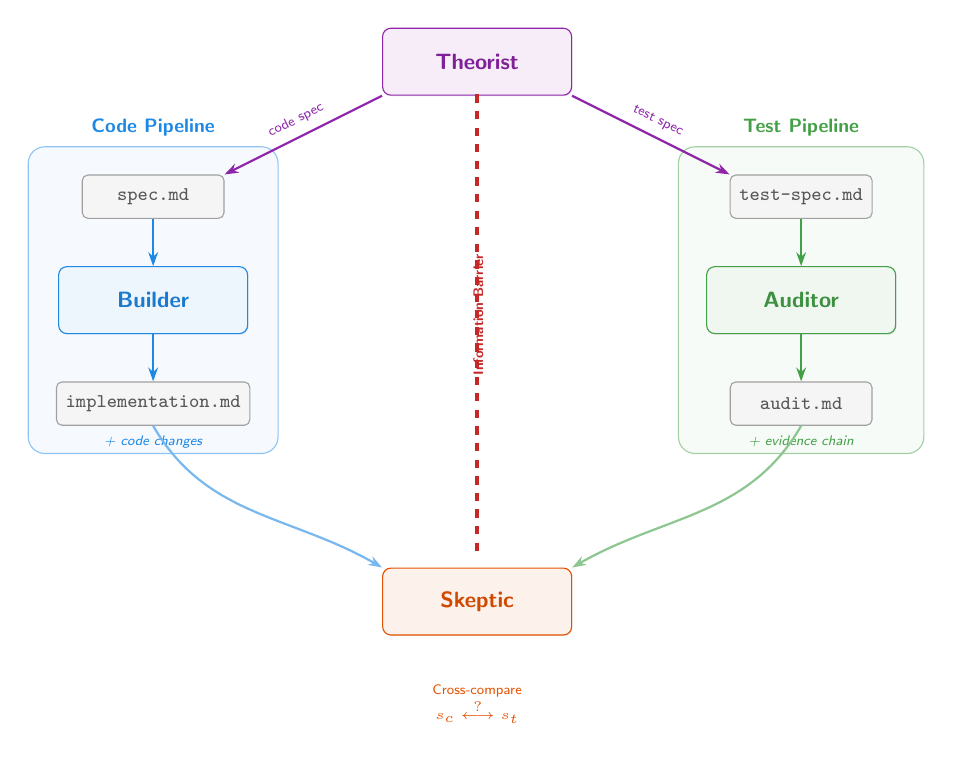
\begin{tikzpicture}[
  node distance=0.7cm and 2.0cm,
  every node/.style={font=\small\sffamily}
]

% ---- Theorist ----
\node[agentbox=cBridge] (theo) {Theorist};

% ---- Two specs ----
\node[artifact, below left=1.0cm and 2.0cm of theo] (spec) {spec.md};
\node[artifact, below right=1.0cm and 2.0cm of theo] (tspec) {test-spec.md};

\draw[arrowstyle=cBridge] (theo.south west) -- (spec.north east)
  node[midway, above, sloped, font=\tiny\sffamily] {code spec};
\draw[arrowstyle=cBridge] (theo.south east) -- (tspec.north west)
  node[midway, above, sloped, font=\tiny\sffamily] {test spec};

% ---- Code pipeline ----
\node[agentbox=cCodePipe, below=0.6cm of spec] (bld) {Builder};
\node[artifact, below=0.6cm of bld] (impl) {implementation.md};
\node[below=0.0cm of impl, font=\tiny\sffamily\itshape, text=cCodePipe]
  {+ code changes};

\draw[arrowstyle=cCodePipe] (spec) -- (bld);
\draw[arrowstyle=cCodePipe] (bld) -- (impl);

% ---- Test pipeline ----
\node[agentbox=cTestPipe, below=0.6cm of tspec] (aud) {Auditor};
\node[artifact, below=0.6cm of aud] (audit) {audit.md};
\node[below=0.0cm of audit, font=\tiny\sffamily\itshape, text=cTestPipe]
  {+ evidence chain};

\draw[arrowstyle=cTestPipe] (tspec) -- (aud);
\draw[arrowstyle=cTestPipe] (aud) -- (audit);

% ---- Barrier ----
\coordinate (mid) at ($(spec.east)!0.5!(tspec.west)$);
\draw[gateline] ($(mid)+(0,1.3)$) -- ($(mid)+(0,-4.5)$);
\node[font=\tiny\sffamily\bfseries, text=cDanger, rotate=90,
      anchor=south] at ($(mid)+(0.2,-1.5)$)
  {Information Barrier};

% ---- Convergence ----
\node[agentbox=cConverge, below=1.8cm of $(impl.south)!0.5!(audit.south)$]
  (skep) {Skeptic};

\draw[arrowstyle=cCodePipe!60] (impl.south) to[out=-60,in=150] (skep.north west);
\draw[arrowstyle=cTestPipe!60] (audit.south) to[out=-120,in=30] (skep.north east);

% convergence annotation
\node[below=0.5cm of skep, font=\tiny\sffamily, text=cConverge,
      align=center] {%
  Cross-compare\\
  $s_c \stackrel{?}{\longleftrightarrow} s_t$%
};

% ---- pipeline boxes ----
\begin{pgfonlayer}{background}
  \node[bigbox=cCodePipe, fit=(spec)(bld)(impl), inner sep=10pt,
        label={[font=\scriptsize\sffamily\bfseries,text=cCodePipe]above:Code Pipeline}] {};
  \node[bigbox=cTestPipe, fit=(tspec)(aud)(audit), inner sep=10pt,
        label={[font=\scriptsize\sffamily\bfseries,text=cTestPipe]above:Test Pipeline}] {};
\end{pgfonlayer}

\end{tikzpicture}
\caption{%
  \textbf{Dual-pipeline artifact flow.}
  Theorist produces two informationally disjoint specifications.
  Builder implements from \texttt{spec.md} without knowledge of test
  scenarios; Auditor validates from \texttt{test-spec.md} without
  knowledge of implementation choices. Skeptic is the sole
  convergence point, cross-comparing both pipelines' outputs.
  The dashed red line denotes the information barrier enforced by
  the Lead at dispatch time.
}
\label{fig:pipeline-detail}
\end{figure}


% =====================================================================
\subsection{Comprehension Verification Protocol}
\label{sec:comprehension}
% =====================================================================

Before producing any specification, the Theorist executes a mandatory
\emph{comprehension verification protocol} that ensures full
understanding of the requirement. This protocol addresses a critical
failure mode in AI-assisted code generation: producing plausible but
mathematically incorrect implementations because the underlying
theory was misunderstood.

The protocol proceeds in four stages:

\begin{enumerate}[leftmargin=*,label=\textbf{Stage \arabic*},itemsep=3pt]
\item \textbf{Inventory.} Catalog all input materials: user prompts,
  uploaded documents (PDF, \LaTeX, handwritten notes), referenced
  papers, and existing code. For each uploaded file, record content
  type (formulas, prose, pseudocode, data) and relevant sections.

\item \textbf{Internalization.} For every mathematical formula:
  restate it in independent notation, define every symbol (type,
  dimensions, domain), list every assumption (identification
  conditions, distributional assumptions, regularity conditions).
  For algorithmic content: specify input/output, step-by-step
  procedure, convergence criteria.

\item \textbf{Self-Test.} Answer six verification questions
  \emph{in writing}:
  \begin{enumerate}[label=(\alph*),itemsep=1pt]
    \item Can the core requirement be restated from memory?
    \item Can every formula be reproduced and each term explained?
    \item Are there any symbols or concepts that cannot be precisely
      defined?
    \item Are there steps requiring judgment not supported by the
      source?
    \item Can the mathematical/statistical intuition be explained?
    \item Are there implicit assumptions the source relies on but
      does not state?
  \end{enumerate}

\item \textbf{Verdict.} Issue \textsc{fully understood} (proceed to
  specification) or \textsc{partially understood} (raise
  \textsc{hold} with targeted questions for the user, up to 3
  rounds).
\end{enumerate}

The comprehension record (\texttt{comprehension.md}) serves as an
auditable evidence trail. Skeptic verifies during convergence review
that specifications are grounded in confirmed understanding, not
speculation.


% =====================================================================
\subsection{State Machine and Hard Gates}
\label{sec:state-machine}
% =====================================================================

Each run follows a deterministic state machine with \emph{hard gate}
preconditions. State transitions are invalid unless all preconditions
are satisfied and verified by artifact inspection.
Figure~\ref{fig:state-machine} shows the state diagram.

\begin{figure}[!t]
\centering
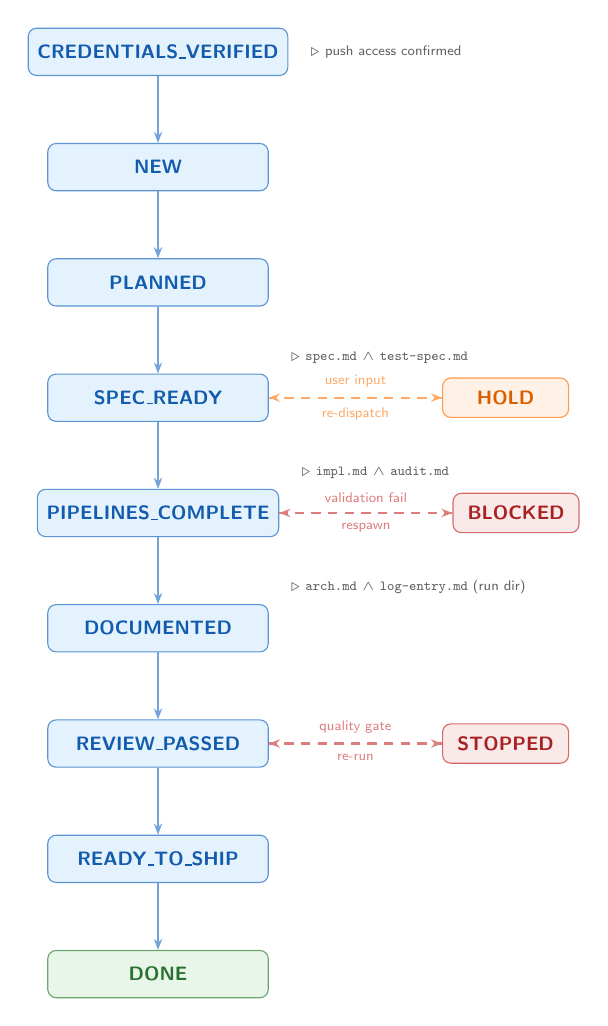
\begin{tikzpicture}[
  node distance=0.85cm,
  state/.style={
    draw=cPrimary!70, fill=cLight, rounded corners=3pt,
    minimum width=2.8cm, minimum height=0.6cm,
    font=\scriptsize\sffamily\bfseries, text=cPrimary!90!black
  },
  interrupt/.style={
    draw=#1!70, fill=#1!10, rounded corners=3pt,
    minimum width=1.6cm, minimum height=0.5cm,
    font=\scriptsize\sffamily\bfseries, text=#1!85!black
  },
  trans/.style={
    -{Stealth[length=4pt, width=3pt]}, thick, color=cPrimary!60
  },
  inttrans/.style={
    -{Stealth[length=4pt, width=3pt]}, thick, color=#1!60, dashed
  },
]

% main states
\node[state] (cred) {CREDENTIALS\_VERIFIED};
\node[state, below=of cred] (new) {NEW};
\node[state, below=of new] (plan) {PLANNED};
\node[state, below=of plan] (spec) {SPEC\_READY};
\node[state, below=of spec] (pipe) {PIPELINES\_COMPLETE};
\node[state, below=of pipe] (doc) {DOCUMENTED};
\node[state, below=of doc] (rev) {REVIEW\_PASSED};
\node[state, below=of rev] (ship) {READY\_TO\_SHIP};
\node[state, below=of ship, draw=cSuccess!70, fill=cLightGreen,
      text=cSuccess!90!black] (done) {DONE};

% main transitions
\foreach \a/\b in {cred/new, new/plan, plan/spec,
  spec/pipe, pipe/doc, doc/rev, rev/ship, ship/done} {
  \draw[trans] (\a) -- (\b);
}

% interrupt states
\node[interrupt=cAccent, right=2.2cm of spec] (hold) {HOLD};
\node[interrupt=cDanger, right=2.2cm of pipe] (block) {BLOCKED};
\node[interrupt=cDanger, right=2.2cm of rev] (stop) {STOPPED};

% interrupt arrows
\draw[inttrans=cAccent] (spec.east) -- (hold.west)
  node[midway, above, font=\tiny\sffamily] {user input};
\draw[inttrans=cAccent] (hold.west) to[out=180,in=0]
  node[midway, below, font=\tiny\sffamily] {re-dispatch} (spec.east);

\draw[inttrans=cDanger] (pipe.east) -- (block.west)
  node[midway, above, font=\tiny\sffamily] {validation fail};
\draw[inttrans=cDanger] (block.west) to[out=180,in=0]
  node[midway, below, font=\tiny\sffamily] {respawn} (pipe.east);

\draw[inttrans=cDanger] (rev.east) -- (stop.west)
  node[midway, above, font=\tiny\sffamily] {quality gate};
\draw[inttrans=cDanger] (stop.west) to[out=180,in=0]
  node[midway, below, font=\tiny\sffamily] {re-run} (rev.east);

% precondition annotations
\node[right=0.15cm of cred.east, font=\tiny\sffamily, text=cGray,
      anchor=west] {$\triangleright$ push access confirmed};
\node[right=0.15cm of spec.north east, font=\tiny\sffamily, text=cGray,
      anchor=south west] {$\triangleright$ \texttt{spec.md} $\wedge$ \texttt{test-spec.md}};
\node[right=0.15cm of pipe.north east, font=\tiny\sffamily, text=cGray,
      anchor=south west] {$\triangleright$ \texttt{impl.md} $\wedge$ \texttt{audit.md}};
\node[right=0.15cm of doc.north east, font=\tiny\sffamily, text=cGray,
      anchor=south west] {$\triangleright$ \texttt{arch.md} $\wedge$ \texttt{log-entry.md} (run dir)};

\end{tikzpicture}
\caption{%
  \textbf{Run state machine with hard gates.}
  Every transition requires artifact-verified preconditions (right
  annotations). Three interrupt states handle distinct failure
  classes: \textsc{hold} (user input needed), \textsc{blocked}
  (validation failure, routed to upstream teammate), and
  \textsc{stopped} (quality gate failure, routed per skeptic's
  verdict). Retry limits (3 cycles per signal) prevent infinite
  loops.
}
\label{fig:state-machine}
\end{figure}

\noindent
Table~\ref{tab:preconditions} formalizes the hard-gate preconditions
for critical state transitions.

\begin{table}[!t]
\centering
\caption{%
  Hard-gate preconditions for state transitions. Each transition
  requires all listed preconditions to be verified by artifact
  inspection before the Lead may update \texttt{status.md}.
}
\label{tab:preconditions}
\small
\begin{tabular}{@{}lp{6.5cm}@{}}
\toprule
\textbf{Target State} & \textbf{Preconditions} \\
\midrule
\textsc{credentials\_verified} &
  \texttt{credentials.md} shows \textsc{pass};
  \texttt{git push --dry-run} succeeded against target repo \\
\textsc{planned} &
  \texttt{request.md} and \texttt{impact.md} exist and are non-empty \\
\textsc{spec\_ready} &
  \texttt{comprehension.md}, \texttt{spec.md}, and
  \texttt{test-spec.md} all exist; Theorist dispatched via Agent tool \\
\textsc{pipelines\_complete} &
  \texttt{implementation.md} and \texttt{audit.md} exist;
  Builder used worktree isolation; pipeline isolation verified
  (Builder prompt $\not\ni$ \texttt{test-spec.md}; Auditor prompt
  $\not\ni$ \texttt{spec.md}); Lead ran no validation commands \\
\textsc{documented} &
  \texttt{Architecture.md} and \texttt{log-entry.md} in run dir;
  Scribe dispatched; github agent syncs to workspace repo \\
\textsc{review\_passed} &
  \texttt{review.md} with verdict \textsc{pass} or
  \textsc{pass with note}; Skeptic dispatched \\
\bottomrule
\end{tabular}
\end{table}


% =====================================================================
\subsection{Signal-Based Error Recovery}
\label{sec:signals}
% =====================================================================

OpenClaw employs exactly three workflow signals, each with a single
exclusive owner, a single meaning, and a single recovery protocol.
This strict signal taxonomy eliminates ambiguity in error handling
and ensures that failures are routed to the correct agent without
human intervention (except when human knowledge is genuinely
required).

\begin{figure}[!t]
\centering
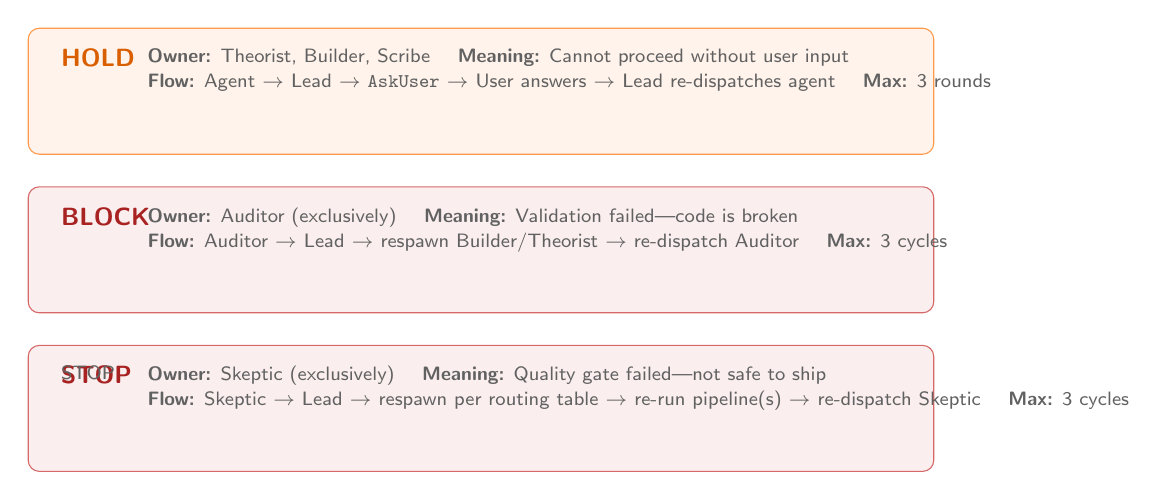
\begin{tikzpicture}[
  node distance=0.4cm and 0.6cm,
  sigblock/.style={
    draw=#1!70, fill=#1!8, rounded corners=4pt,
    minimum width=11.5cm, minimum height=1.6cm,
    inner sep=6pt
  },
  siglabel/.style={
    font=\small\sffamily\bfseries, text=#1!85!black
  },
  sigdesc/.style={
    font=\scriptsize\sffamily, text=cGray, align=left
  },
]

% HOLD
\node[sigblock=cAccent] (holdbox) {};
\node[siglabel=cAccent, anchor=north west] at
  ($(holdbox.north west)+(0.3,-0.15)$) {HOLD};
\node[sigdesc, anchor=north west] at
  ($(holdbox.north west)+(1.4,-0.15)$) {%
  \textbf{Owner:} Theorist, Builder, Scribe \quad
  \textbf{Meaning:} Cannot proceed without user input\\[1pt]
  \textbf{Flow:} Agent $\to$ Lead $\to$ \texttt{AskUser} $\to$
  User answers $\to$ Lead re-dispatches agent \quad
  \textbf{Max:} 3 rounds%
};

% BLOCK
\node[sigblock=cDanger, below=0.4cm of holdbox] (blockbox) {};
\node[siglabel=cDanger, anchor=north west] at
  ($(blockbox.north west)+(0.3,-0.15)$) {BLOCK};
\node[sigdesc, anchor=north west] at
  ($(blockbox.north west)+(1.4,-0.15)$) {%
  \textbf{Owner:} Auditor (exclusively) \quad
  \textbf{Meaning:} Validation failed---code is broken\\[1pt]
  \textbf{Flow:} Auditor $\to$ Lead $\to$ respawn Builder/Theorist
  $\to$ re-dispatch Auditor \quad
  \textbf{Max:} 3 cycles%
};

% STOP
\node[sigblock=cDanger, below=0.4cm of blockbox] (stopbox) {};
\node[siglabel=cDanger, anchor=north west] at
  ($(stopbox.north west)+(0.3,-0.15)$) {STOP};
\node[sigdesc, anchor=north west] at
  ($(stopbox.north west)+(0.3,-0.15)$) {STOP};
\node[sigdesc, anchor=north west] at
  ($(stopbox.north west)+(1.4,-0.15)$) {%
  \textbf{Owner:} Skeptic (exclusively) \quad
  \textbf{Meaning:} Quality gate failed---not safe to ship\\[1pt]
  \textbf{Flow:} Skeptic $\to$ Lead $\to$ respawn per routing table
  $\to$ re-run pipeline(s) $\to$ re-dispatch Skeptic \quad
  \textbf{Max:} 3 cycles%
};

\end{tikzpicture}
\caption{%
  \textbf{Signal taxonomy and recovery protocols.}
  Each signal has one exclusive owner, one semantic meaning, and one
  deterministic recovery path. \textsc{hold} requires human input;
  \textsc{block} and \textsc{stop} are resolved autonomously by
  respawning the responsible teammate. A retry limit of 3 cycles
  per signal prevents infinite loops; exhaustion escalates to
  \textsc{hold}.
}
\label{fig:signals}
\end{figure}

Key design properties of the signal system:

\begin{itemize}[leftmargin=*,itemsep=2pt]
  \item \textbf{Non-overlapping ownership.} Each signal has exactly
    one owner agent, eliminating ambiguity about who may raise which
    signal.
  \item \textbf{Autonomous recovery.} \textsc{block} and
    \textsc{stop} are resolved without user interaction---the Lead
    respawns the responsible upstream teammate and re-validates.
  \item \textbf{Bounded retry.} Each signal type permits at most 3
    recovery cycles. Exhaustion escalates to \textsc{hold}, ensuring
    the system always terminates.
  \item \textbf{No nesting.} A \textsc{block} cannot trigger a
    \textsc{stop}, and vice versa. Each signal is handled
    independently within its recovery protocol.
\end{itemize}


% =====================================================================
\subsection{Tolerance Integrity and Anti-Fraud Mechanisms}
\label{sec:tolerance}
% =====================================================================

A subtle but critical failure mode in AI-driven validation is
\emph{tolerance inflation}: the validating agent silently widens
numerical thresholds to convert genuine failures into false passes.
OpenClaw addresses this through a multi-layered defense:

\begin{enumerate}[leftmargin=*,label=(\roman*),itemsep=3pt]
  \item \textbf{Specification-locked tolerances.} All numerical
    tolerances ($\texttt{atol}$, $\texttt{rtol}$, $\epsilon$) are
    defined exclusively in \texttt{test-spec.md} by the Theorist.
    The Auditor \emph{must not} modify these values.

  \item \textbf{Evidence recording.} The Auditor must record in
    \texttt{audit.md} the exact tolerance used for every numerical
    comparison alongside the value specified in
    \texttt{test-spec.md}, enabling line-by-line cross-referencing.

  \item \textbf{Skeptic cross-audit.} The Skeptic performs a
    mandatory tolerance integrity audit (Step~7a of its protocol),
    cross-referencing every tolerance in \texttt{audit.md} against
    \texttt{test-spec.md}. Any discrepancy triggers an immediate
    \textsc{stop}.

  \item \textbf{Evasion pattern detection.} The Skeptic checks for
    additional manipulation patterns: removed assertions,
    \texttt{try/catch} wrappers around failing checks, reduced
    iteration counts, unjustified seed changes, and silent scenario
    omissions.
\end{enumerate}

\noindent
This defense-in-depth ensures that the only valid response to a
genuinely failing test is \textsc{block}---never silent tolerance
relaxation.


% =====================================================================
\subsection{Worktree Isolation and Concurrent Execution}
\label{sec:worktree}
% =====================================================================

OpenClaw distinguishes between two levels of isolation:

\paragraph{Information-level isolation} (Section~\ref{sec:dual-pipeline})
prevents cross-contamination of specifications between the code and
test pipelines.

\paragraph{Filesystem-level isolation} prevents concurrent writers
from corrupting each other's working copy. Any agent that modifies
files in the target repository (Builder, Scribe) is dispatched with
\texttt{isolation: "worktree"}, which creates a temporary git
worktree---an independent checkout of the same repository. Changes
are merged back to the main checkout upon completion.

This two-level isolation enables the critical \emph{parallel dispatch}
optimization: Builder and Auditor are dispatched in the same message.
Builder writes code in its worktree; Auditor prepares validation
scenarios concurrently. When Builder's worktree merges back, Auditor
runs its validation on the merged result. The dispatch is parallel;
the validation targets the merged state.


% =====================================================================
\subsection{Workflow Catalog}
\label{sec:workflows}
% =====================================================================

OpenClaw supports nine workflow types, selected by the Lead through
semantic intent detection from natural language prompts.
Table~\ref{tab:workflows} summarizes the agent sequences.

\begin{table}[!t]
\centering
\caption{%
  Workflow catalog. Notation: ``$\parallel$'' denotes parallel
  dispatch; ``$\to$'' denotes sequential; ``?'' denotes conditional
  activation. Workflows 6--8 are lightweight exceptions that
  intentionally skip the full two-pipeline flow.
}
\label{tab:workflows}
\small
\begin{tabular}{@{}clp{6cm}@{}}
\toprule
\textbf{\#} & \textbf{Name} & \textbf{Agent Sequence} \\
\midrule
1 & Standard &
  Lead $\to$ Theorist $\to$ [Builder $\parallel$ Auditor]
  $\to$ Scribe $\to$ Skeptic \\
2 & With Docs &
  Lead $\to$ Theorist $\to$ [Builder $\parallel$ Auditor]
  $\to$ Scribe $\to$ Skeptic \\
3 & With Ship &
  Lead $\to$ Theorist $\to$ [Builder $\parallel$ Auditor]
  $\to$ Scribe $\to$ Skeptic $\to$ GitHub \\
4 & Issue Patrol &
  Lead scans $\to$ per issue: full pipeline $\to$ GitHub \\
5 & Single Issue &
  Lead $\to$ full pipeline $\to$ GitHub \\
6 & Validation Only &
  Lead $\to$ Auditor \\
7 & Ship Only &
  Lead $\to$ Skeptic $\to$ GitHub \\
8 & Review Only &
  Lead $\to$ Skeptic \\
9 & Scheduled Loop &
  Lead $\to$ \texttt{/loop} $\to$ inner workflow \\
\bottomrule
\end{tabular}
\end{table}


% =====================================================================
\subsection{Artifact Graph and Handoff Protocol}
\label{sec:artifacts}
% =====================================================================

All inter-agent communication is mediated through typed Markdown
artifacts stored in a structured run directory
(\texttt{.statsclaw/runs/<id>/}). Agents never communicate directly;
every handoff flows through the Lead:
\[
  A_{\text{upstream}} \;\xrightarrow{\text{artifact}}\;
  \text{Lead reads} \;\xrightarrow{\text{dispatch}}\;
  A_{\text{downstream}} \;\xrightarrow{\text{reads artifact}}\;
  \text{executes}
\]
This mediated handoff enables the Lead to enforce pipeline isolation
at every transition, verify artifact existence before dispatch, and
inject failure context when respawning agents after \textsc{block}
or \textsc{stop} signals.

Figure~\ref{fig:artifact-flow} shows the complete artifact dependency
graph across a standard workflow run.

\begin{figure}[!t]
\centering
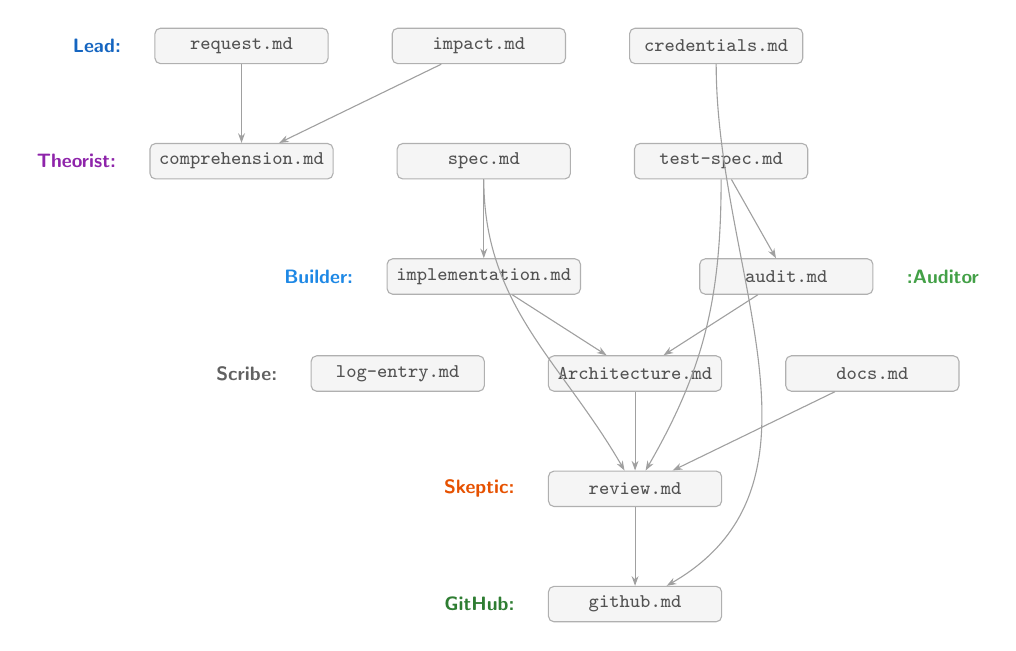
\begin{tikzpicture}[
  node distance=0.6cm and 0.8cm,
  art/.style={
    draw=cGray!50, fill=cLightGray, rounded corners=2pt,
    minimum width=2.2cm, minimum height=0.45cm,
    font=\scriptsize\ttfamily, text=cGray!85!black
  },
  ag/.style={
    font=\scriptsize\sffamily\bfseries, text=#1
  },
  fl/.style={
    -{Stealth[length=3.5pt, width=2.5pt]}, color=cGray!60, thin
  },
]

% row 1: lead artifacts
\node[art] (req) {request.md};
\node[art, right=of req] (imp) {impact.md};
\node[art, right=of imp] (cred) {credentials.md};
\node[ag=cPrimary, left=0.3cm of req] {Lead:};

% row 2: theorist artifacts
\node[art, below=1.0cm of req] (comp) {comprehension.md};
\node[art, right=of comp] (spec) {spec.md};
\node[art, right=of spec] (tspec) {test-spec.md};
\node[ag=cBridge, left=0.3cm of comp] {Theorist:};

% row 3: pipeline outputs
\node[art, below=1.0cm of spec] (implmd) {implementation.md};
\node[art, right=1.5cm of implmd] (auditmd) {audit.md};
\node[ag=cCodePipe, left=0.3cm of implmd] {Builder:};
\node[ag=cTestPipe, right=0.3cm of auditmd] {:Auditor};

% row 4: scribe
\node[art, below=1.0cm of $(implmd)!0.5!(auditmd)$] (arch) {Architecture.md};
\node[art, left=of arch] (logmd) {log-entry.md};
\node[art, right=of arch] (docs) {docs.md};
\node[ag=cGray, left=0.3cm of logmd] {Scribe:};

% row 5: skeptic
\node[art, below=1.0cm of arch] (review) {review.md};
\node[ag=cConverge, left=0.3cm of review] {Skeptic:};

% row 6: github
\node[art, below=1.0cm of review] (ghmd) {github.md};
\node[ag=cSuccess, left=0.3cm of ghmd] {GitHub:};

% dependency arrows
\draw[fl] (req) -- (comp);
\draw[fl] (imp) -- (comp);
\draw[fl] (spec) -- (implmd);
\draw[fl] (tspec) -- (auditmd);
\draw[fl] (implmd) -- (arch);
\draw[fl] (auditmd) -- (arch);
\draw[fl] (arch) -- (review);
\draw[fl] (docs) -- (review);
\draw[fl] (spec) to[out=-90,in=120] (review);
\draw[fl] (tspec) to[out=-90,in=60] (review);
\draw[fl] (review) -- (ghmd);
\draw[fl] (cred) to[out=-90,in=30] (ghmd);

\end{tikzpicture}
\caption{%
  \textbf{Artifact dependency graph.}
  Each row shows one agent's output artifacts and their dependencies
  on upstream artifacts. Arrows indicate ``reads before producing.''
  The Lead mediates every transition, enforcing pipeline isolation
  by ensuring Builder never receives \texttt{test-spec.md} and
  Auditor never receives \texttt{spec.md}.
}
\label{fig:artifact-flow}
\end{figure}


% =====================================================================
\subsection{Mailbox Protocol and Asynchronous Communication}
\label{sec:mailbox}
% =====================================================================

A shared, append-only mailbox (\texttt{mailbox.md}) in each run
directory provides a communication channel for agents to report
interface changes, request user input, or leave informational notes
for downstream teammates. The mailbox supports three message types:

\begin{itemize}[leftmargin=*,itemsep=2pt]
  \item \texttt{INFO}: Non-blocking observation (e.g., a judgment
    call made during implementation).
  \item \texttt{HOLD\_REQUEST}: Corresponds to a \textsc{hold}
    signal; the Lead forwards the question to the user.
  \item \texttt{INTERFACE\_CHANGE}: A function signature, export, or
    file path changed; the Lead notifies affected downstream agents.
\end{itemize}

\noindent
The append-only constraint ensures a reliable audit trail: messages
are never deleted, edited, or reordered, providing a complete
chronological record of inter-agent communication that the Scribe
captures in the process-record log entry.


% =====================================================================
\subsection{Process Recording and Traceability}
\label{sec:recording}
% =====================================================================

The Scribe agent produces two mandatory artifacts that create a
persistent institutional memory for the target repository:

\paragraph{Architecture diagram (\texttt{Architecture.md}).}
A system-level view of the codebase rendered as Mermaid diagrams:
module structure with layer groupings, function call graphs tracing
public entry points to internal helpers, and data-flow charts with
decision diamonds. Changed modules are visually highlighted. This
artifact stays in the local run directory for reviewer verification---it
is \emph{not} synced to the workspace repo or committed to the target
repository, keeping both clean.

\paragraph{Process-record log (\texttt{log-entry.md}).}
A chronological log entry capturing the entire workflow: Theorist's
proposals, Builder's implementation decisions, Auditor's validation
results with exact tolerances, all \textsc{block}/\textsc{hold}/\textsc{stop}
signals and their resolutions, and Skeptic's review verdict. Log
entries are synced to the workspace repository
(\texttt{[owner]/workspace/<repo>/runs/}) as a traceable record of
all code changes, enabling any future developer to understand not
just \emph{what} changed, but \emph{why} and \emph{how it was
verified}. The workspace repo accumulates logs across all target
repositories in one place.


% =====================================================================
\subsection{Multi-Language Support via Profiles}
\label{sec:profiles}
% =====================================================================

OpenClaw is language-agnostic by design. Language-specific conventions
are encapsulated in \emph{profiles}---declarative configuration files
that specify validation commands, documentation conventions, package
manifest formats, and release exclusion patterns.
Table~\ref{tab:profiles} lists the currently supported profiles.

\begin{table}[!t]
\centering
\caption{%
  Language profiles supported by OpenClaw. Each profile defines
  validation commands, documentation conventions, and release
  exclusion patterns for development-only artifacts.
}
\label{tab:profiles}
\small
\begin{tabular}{@{}llll@{}}
\toprule
\textbf{Profile} & \textbf{Validation Command} &
  \textbf{Doc System} & \textbf{Workflow Logs} \\
\midrule
R Package     & \texttt{R CMD check --as-cran}  & roxygen2
  & workspace repo \\
Python        & \texttt{pytest --tb=short}      & docstrings/Sphinx
  & workspace repo \\
TypeScript    & \texttt{npm test}               & JSDoc/TSDoc
  & workspace repo \\
Go Module     & \texttt{go test ./...}          & godoc
  & workspace repo \\
Rust Crate    & \texttt{cargo test}             & rustdoc
  & workspace repo \\
Stata         & \texttt{do run\_tests.do}       & SMCL help files
  & workspace repo \\
\bottomrule
\end{tabular}
\end{table}

\noindent
Profile detection is automatic: the Lead inspects repository markers
(\texttt{DESCRIPTION} for R, \texttt{pyproject.toml} for Python,
\texttt{package.json} for TypeScript, \texttt{go.mod} for Go,
\texttt{Cargo.toml} for Rust) and selects the appropriate profile.
Mixed-language repositories may activate multiple profiles.


% =====================================================================
\subsection{Discussion: Design Principles}
\label{sec:design-principles}
% =====================================================================

We conclude by summarizing the core design principles that
distinguish OpenClaw from prior AI-assisted development frameworks:

\begin{enumerate}[leftmargin=*,label=\textbf{P\arabic*.},itemsep=4pt]
  \item \textbf{Adversarial verification by construction.}
    The dual-pipeline architecture ensures that implementation and
    validation are derived independently from the same requirement.
    Convergence of two independent derivations provides stronger
    correctness evidence than any single-pipeline approach
    (Equation~\ref{eq:false-positive}).

  \item \textbf{Comprehension before specification.}
    The mandatory comprehension verification protocol
    (Section~\ref{sec:comprehension}) prevents a common failure mode
    in AI code generation: producing syntactically valid but
    semantically incorrect code due to misunderstood requirements.

  \item \textbf{Hard gates, not soft advice.}
    State transitions are guarded by artifact-verified preconditions
    (Table~\ref{tab:preconditions}). The system physically cannot
    advance past a failed gate, unlike advisory checklists that can
    be ignored.

  \item \textbf{Tolerance integrity as a first-class concern.}
    The anti-fraud mechanisms of Section~\ref{sec:tolerance} address
    a novel threat in AI-driven validation: the validating agent
    silently relaxing thresholds to produce false passes.

  \item \textbf{Mediated communication only.}
    All inter-agent handoffs flow through the Lead
    (Section~\ref{sec:artifacts}), enabling centralized isolation
    enforcement and complete audit trails.

  \item \textbf{Bounded autonomous recovery.}
    The three-signal system (Section~\ref{sec:signals}) enables
    autonomous error recovery while guaranteeing termination through
    retry limits.

  \item \textbf{Institutional memory.}
    Process-record logs (Section~\ref{sec:recording}) capture not
    just what changed but the full decision trail---proposals,
    validations, failures, and resolutions---creating a traceable
    history that persists beyond any single AI session.
\end{enumerate}
